% !TEX root = ../main.tex
\section{Method}

\subsection{Design}

\begin{table}
\begin{adjustbox}{width=\columnwidth}
\begin{tabular}{llll}
\hline
\textbf{Name}      & \textbf{Short} & \textbf{Sequence}                                           & \textbf{Length} \\
\hline
T7 promoter        & 0          & GGTAATACGACTCACTATAG                                           & 20     \\
Short 1            & 1          & CCTCAAGGAGCTTCAGTCTAGCCCTATAGTGAGTCGTATTACC                    & 43     \\
Short 2            & 2          & CTCCTTGAGGCACATAACTCCCCTATAGTGAGTCGTATTACC                     & 42     \\
Short 3            & 3          & CACATAACTCTACTAAATCTCCCTATAGTGAGTCGTATTACC                     & 42     \\
Short 4            & 4          & GAGTTATGTGCCTCAAGGAGCCCTATAGTGAGTCGTATTACC                    & 42     \\
Short 5            & 5          & AGATTTAGTAGAGTTATGTGCCCTATAGTGAGTCGTATTACC                     & 42     \\
Long 1             & 6          & GTCAATTCGCCTCAAGGAGCTTCAGTCTAGCCCTATAGTGAGTCGTATTACC           & 52     \\
Long 2             & 7          & GCTCCTTGAGGCGAATTGACCCATCTTCATTCTACTCCTACCCTATAGTGAGTCGTATTACC & 62     \\
Long 3             & 8          & CCATCTTCATTCTACTCCTATACCTCAATCCCCTATAGTGAGTCGTATTACC           & 52     \\
Long 4             & 9          & TAGGAGTAGAATGAAGATGGGTCAATTCGCCTCAAGGAGCCCCTATAGTGAGTCGTATTACC & 62     \\
Long 5             & 10         & GATTGAGGTATAGGAGTAGAATGAAGATGGCCCTATAGTGAGTCGTATTACC           & 52     \\
% Beacon fluorophore & 11         & CGGCTAGACTGAA                                                  & 13     \\
% Beacon quencher    & 12         & CCTCAAGGAGCTTCAGTCTAGCCG                                       & 24 \\
\hline
\end{tabular}
\end{adjustbox}
\caption{Sequences and names of the DNA strands used for transcription.}
\label{dna_strands}
\end{table}

\begin{table}
\begin{adjustbox}{width=\columnwidth}
\begin{tabular}{llll}
\hline
\textbf{Name}      & \textbf{Short} & \textbf{Sequence}                                           & \textbf{Length} \\
\hline
Short 1            & 1          & GGCUAGACUGAAGCUCCUUGAGG                    & 23     \\
Short 2            & 2          & GGGAGUUAUGUGCCUCAAGGAG                     & 22     \\
Short 3            & 3          & GGAGAUUUAGUAGAGUUAUGUG                     & 22     \\
Short 4            & 4          & GGCUCCUUGAGGCACAUAACUC                     & 22     \\
Short 5            & 5          & GGCACAUAACUCUACUAAAUCU                     & 22     \\
Long 1             & 6          & GGCUAGACUGAAGCUCCUUGAGGCGAAUUGAC           & 32     \\
Long 2             & 7          & GGUAGGAGUAGAAUGAAGAUGGGUCAAUUCGCCUCAAGGAGC & 42     \\
Long 3             & 8          & GGGAUUGAGGUAUAGGAGUAGAAUGAAGAUGG           & 32     \\
Long 4             & 9          & GGGCUCCUUGAGGCGAAUUGACCCAUCUUCAUUCUACUCCUA & 42     \\
Long 5             & 10         & GGCCAUCUUCAUUCUACUCCUAUACCUCAAUC           & 32     \\
% Beacon fluorophore & 11         & CGGCTAGACTGAA                                                  & 13     \\
% Beacon quencher    & 12         & CCTCAAGGAGCTTCAGTCTAGCCG                                       & 24 \\
\hline
\end{tabular}
\end{adjustbox}
\caption{Sequences and names of the transcribed RNA strands.}
\label{rna_strands}
\end{table}

\subsection{Transcription}

The oligos from IDT was dissolved in TE buffer [PROTOCOL] to an approximate concentration of 120 $\mu$M, based on the quantity of substance written on the tubes. The final concentration desired was 100 $\mu$M, but due to a risk of inaccurate substance quantities, the dissolved concentration was chosen to be slightly above. The oligos could then be further diluted after measuring their absorbance on the Nanodrop.

After dissolving the oligos, the absorbance of each sample was measured on the Nanodrop in triplets. A program was written which can take the .csv output of the Nanodrop, and calculate the concentration based on each strands extinction coefficient \cite{nanodropimport}.

The measured concentrations (figure \ref{oligo_concentrations}) was used to dilute the samples further, to a concentration of 100 $\mu$M.

To anneal the templates to the promoter, each of the template strands was mixed with equal amounts of promoter strand in annealing buffer [PROTOCOL], to a final concentration of 1 $\mu$M. The mixed samples were then heated to 90$^\circ$ C for 5 minutes, and left to cool down to room temperature.

To check if samples annealed properly, they were run on a 20\% native PAGE gel for 3 hours. Each lane was loaded with 50 $\mu$l sample, and 10 $\mu$l native loading buffer [PROTOCOL]. Afterwards the gel was stained in SYBR Gold, and visualised on the Typhoon scanner [PROTOCOL]. The result of the scan can be seen in figure \ref{fig:promoter_annealing_gel}.

\begin{figure}[H]
\centering
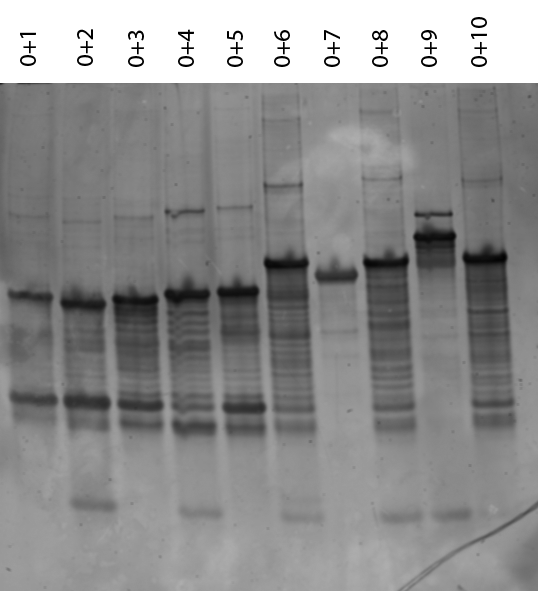
\includegraphics[width=\columnwidth]{images/promoter_annealing_gel.png}
\caption{Typhoon scan of SYBR Gold stained native PAGE gel, with the annealed templates and promoter strands. The lanes are labelled by which strands are annealed (see table \ref{dna_strands}).}
\label{fig:promoter_annealing_gel}
\end{figure}

As can be seen in figure \ref{fig:promoter_annealing_gel}, the darkest bands is the annealed samples. The samples for the short translator runs as about the same size, while there is bigger variation in the long translator samples, as expected based on table \ref{dna_strands}. The exact positions of the long translator samples does not match with the sequence length, though this can be explained by secondary structures of the single-stranded part of the sample. The shorter bands visible below, is probably excess promoter, other secondary structures, and shorter sequences from synthesis errors. No lane with ladder was run, so the exact position of the bands can't be commented on.

To get the desired RNA sequences, a transcription reaction was run with each of the annealed DNA templates, according to table \ref{transcription1}.

\begin{table}\centering
\begin{tabular}{llll}
  \hline
                       & \textbf{Initial conc.} & \textbf{Final conc.} & \textbf{Volume} \\ \hline
  Transcription buffer & 10X                    & 1X                   & 10 \si{\micro}L           \\
  DTT                  & 100 mM                 & 10 mM                & 10 \si{\micro}L           \\
  NTP mix              & 25 mM                  & 2.5 mM               & 10 \si{\micro}L           \\
  Template             & 500 nM                 & 50 nM                & 10 \si{\micro}L           \\
  T7 RNA polymerase    &                        &                      & 1 \si{\micro}L            \\
  Nuclease-free water  &                        &                      & 59 \si{\micro}L           \\
  Total                &                        &                      & 100 \si{\micro}L          \\ \hline
\end{tabular}
\caption{Mixing of compounds for the first transcription done on the templates for both the short and long translater.}
\label{transcription1}
\end{table}

The samples were left overnight at 37$^\circ$ C. The day after, 1 \si{\micro}L of RNAse free DNAse was added to the samples, and heated for 37$^\circ$ C for an hour. Afterwards, 100 ul of denaturing loading buffer was added to each sample, and 10 ul of the DNA 0 and DNA 5 strands was mixed with 10 ul of denaturing loading buffer, and heated for 5 minutes at 90$^\circ$ C.

To purify the RNA, the transcribed sequences and controls were run on a 20\% denaturing PAGE gel, for 4 hours at 20 W.

The RNA product should be visible in UV shadowing, but no product was visible. The gel was then stained with SYBR Gold and scanned on the Typhoon [PROTOCOL]. The result can be seen in figure \ref{transcription_1}.

\begin{figure}[H]
\centering
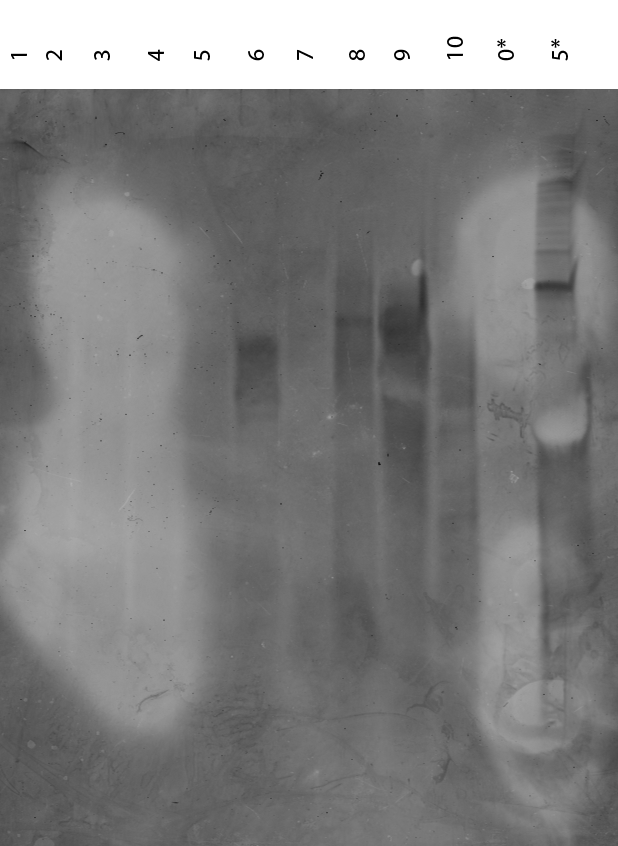
\includegraphics[width=200]{images/translator_transcription_1.png}
\caption{Typhoon scan of SYBR Gold stained native PAGE gel, with the transcribed RNA strands in lanes 1-10, and controls in 11 and 12. The lanes are labelled by which strands are annealed (see \tref{rna_strands}). The asterix refers to the DNA strands in \tref{dna_strands}.}
\label{transcription_1}
\end{figure}

As can be seen in \fref{transcription_1}, the gel wasn't stained long enough, so after restaining it in SYBR Gold, it was scanned again.

\begin{figure}[H]
\centering
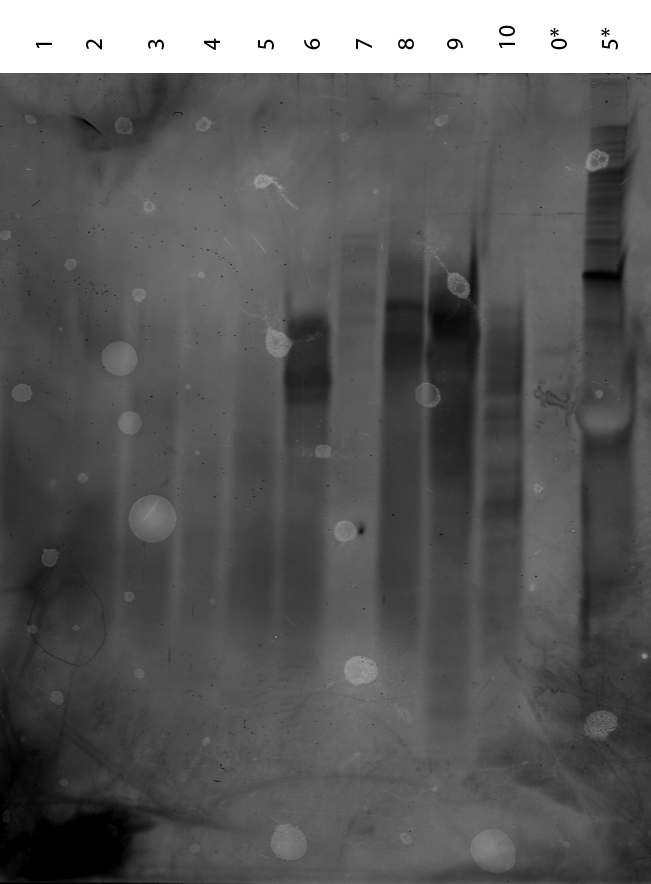
\includegraphics[width=200]{images/translator_transcription_2.png}
\caption{Typhoon scan of SYBR Gold stained native PAGE gel, with the transcribed RNA strands in lanes 1-10, and controls in 11 and 12. The lanes are labelled by which strands are annealed (see table \ref{rna_strands}). The asterix refers to the DNA strands in table \ref{dna_strands}.}
\label{transcription_2}
\end{figure}

The lanes 1-10 in \fref{transcription_2} does not show distinct bands. There seems to be more product from the long translator transcriptions (lanes 6-10), than in the short ones (lanes 1-5). Even the controls which were loaded in equal amounts does not show up in equal strength. Since the gel from the DNA annealing was run without any controls, it was difficult to see if there was any errors in the annealing. Another 20\% native PAGE gel was run with the annealed DNA, using the single stranded oligos as control. To simplify the experiment while trying to the find the error, only the short translator sequences were used.

\begin{figure}[H]
\centering
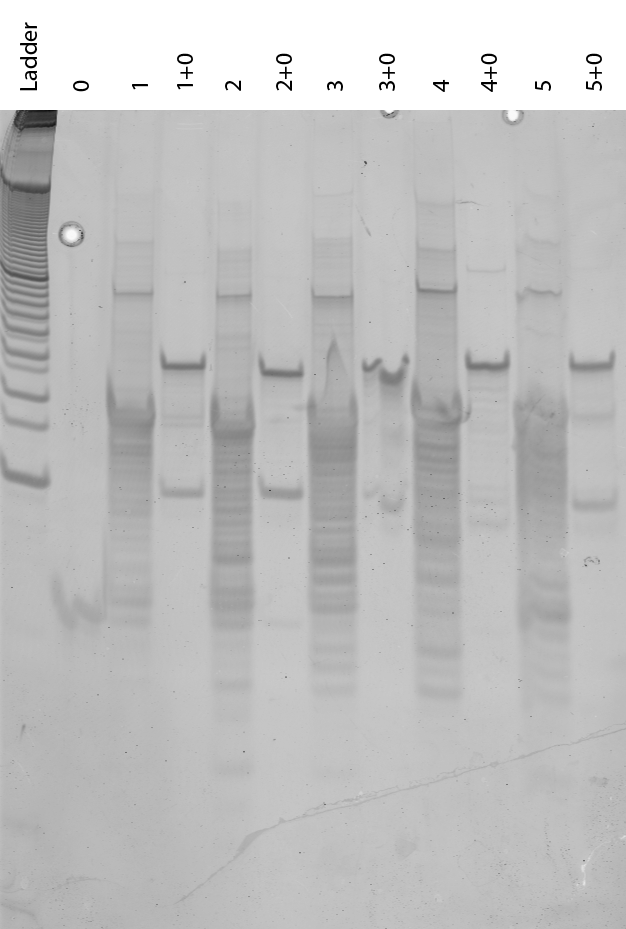
\includegraphics[width=200]{images/translator_annealing_2.png}
\caption{The annealed oligos together with controls and a 10 nt ladder. The lanes are labelled with the oligo names given in \tref{dna_strands}. The plus symbol denotes which strands are annealed.}
\label{translator_annealing_2}
\end{figure}

The results of \fref{translator_annealing_2} still shows that the templates have annealed with the promoter, and runs as about 40-50 bp. The expected size is around 60 bp (sum of promoter and template), but it is difficult to say how a partly annealed structure will run on a native gel. The new gel does however show that the bands in the annealed lanes below the assumed product, might not be excess promoter. The promoter is seen in the second lane, and lies below the bands in the annealed structure thought to be excess promoter. The bands below the product might be due to secondary structures of each of the template strands, but comparing with \fref{short_secondary_structures}, the band in the 5+0 lane would be expected to be less visible, as strand 5 has no secondary structure.

Despite the unexplained bands from the annealing, a new transcription was run on the short template strands to see if better results could be attained.
